\subsection{The definite integral as signed area}

For a non-negative function, the definite integral measures the area between the graph and the horizontal axis. The picture below represents
\[
\int_0^2 x^2\,dx.
\]

\begin{center}
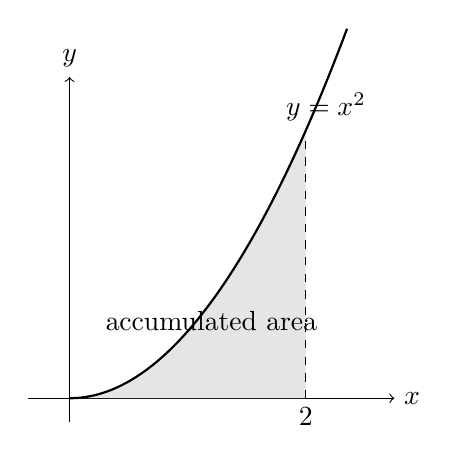
\begin{tikzpicture}[x=1.5cm,y=0.85cm]
  \draw[->] (-0.35,0) -- (2.75,0) node[right] {$x$};
  \draw[->] (0,-0.35) -- (0,4.8) node[above] {$y$};
  \fill[gray!20] (0,0) -- plot[domain=0:2,samples=80] (\x,{\x*\x}) -- (2,0) -- cycle;
  \draw[thick,domain=0:2.35,samples=80] plot (\x,{\x*\x});
  \draw[dashed] (2,0) -- (2,4);
  \node[below] at (2,0) {$2$};
  \node at (1.2,1.15) {accumulated area};
  \node[anchor=west] at (1.75,4.35) {$y=x^2$};
\end{tikzpicture}
\end{center}

\begin{interpretationbox}[The integral adds vertical contributions]
Each narrow vertical strip has approximate area $f(x)\,\Delta x$. The definite integral is the limiting total of these strips as their widths become smaller.
\end{interpretationbox}
